% Defense visual system copied from the approved study deck.
% Evidence labels and scopes are defined in main.tex and CLAIMS.md.
\documentclass[aspectratio=169,12pt,t]{beamer}

% Speaker notes: uncomment ONE line to see them.
% \setbeameroption{show notes on second screen=right}  % dual-screen (pdfpc)
% \setbeameroption{show only notes}                     % notes handout

\usetheme[progressbar=none, sectionpage=none]{moloch}
% A 208 x 117 mm canvas retains 16:9 and the actual 12pt class fonts.
% Long owner-approved sentences fit without frame scaling or reduced fonts.
\geometry{paperwidth=208mm,paperheight=117mm}

% ---------- fonts ----------
\usepackage{fontspec}
\setsansfont{Avenir Next}[BoldFont={Avenir Next Demi Bold}]
\setmonofont{Menlo}[Scale=1.0]
\newcommand{\captiontype}{\small}

% ---------- palette ----------
\definecolor{navy}{HTML}{1F3A5F}
\definecolor{teal}{HTML}{2A9D8F}
\definecolor{fault}{HTML}{E76F51}
\definecolor{paper}{HTML}{FAFAF7}
\definecolor{ink}{HTML}{22262B}
\definecolor{muted}{HTML}{6B7280}
\definecolor{rule}{HTML}{D6D9DE}

\setbeamercolor{normal text}{fg=ink, bg=paper}
\setbeamercolor{frametitle}{fg=paper, bg=navy}
\setbeamercolor{progress bar}{fg=teal, bg=rule}
\setbeamercolor{alerted text}{fg=fault}
\setbeamercolor{example text}{fg=teal}
\setbeamercolor{structure}{fg=navy}
\setbeamercolor{title separator}{fg=teal}
\setbeamercolor{footline}{fg=muted}
% Beamer otherwise inherits the fault/alert color for in-slide citations.
\setbeamercolor{bibliography entry author}{fg=navy}
\setbeamercolor{bibliography entry title}{fg=ink}
\setbeamercolor{bibliography entry location}{fg=muted}
\setbeamercolor{bibliography entry note}{fg=muted}
\setbeamercolor{block title}{fg=paper, bg=navy}
\setbeamercolor{block body}{bg=navy!6}
\setbeamerfont{frametitle}{size=\large, series=\bfseries}
\setbeamertemplate{frametitle}{\nointerlineskip\begin{beamercolorbox}[wd=\paperwidth,sep=2mm,leftskip=4mm]{frametitle}\usebeamerfont{frametitle}\insertframetitle\strut\end{beamercolorbox}}
\setbeamertemplate{itemize items}{\color{teal}\rule[0.25ex]{0.45em}{0.45em}}
\setbeamertemplate{bibliography item}[text]
\setbeamertemplate{page number in head/foot}[totalframenumber]
\hypersetup{colorlinks=true, linkcolor=navy, urlcolor=navy, citecolor=navy}
% Keep the appendix bookmark free of Beamer translation commands.
\pdfstringdefDisableCommands{\def\translate#1{#1}}

\setbeamertemplate{itemize subitem}{\color{muted}--}

% ---------- packages ----------
\usepackage{tikz}
\usetikzlibrary{arrows.meta, positioning, automata, calc, shapes.geometric, fit, backgrounds, decorations.pathreplacing}
\usepackage{booktabs}
\usepackage{array}
\newcolumntype{L}[1]{>{\raggedright\arraybackslash}p{#1}}
\usepackage{amsmath}
\usepackage{siunitx}
\sisetup{detect-all}

% ---------- helpers ----------
\newcommand{\muted}[1]{{\color{muted}#1}}

% \slideimg[<max height>]{<width>}{<V-id>}{<caption for placeholder>}
% Shows images/<V-id>.jpg or .png if present, otherwise a labelled gray box of the same size.
\newcommand{\slideimg}[4][0.64\textheight]{%
  \IfFileExists{images/#3.jpg}{%
    \includegraphics[width=#2, height=#1, keepaspectratio]{images/#3.jpg}%
  }{\IfFileExists{images/#3.png}{%
    \includegraphics[width=#2, height=#1, keepaspectratio]{images/#3.png}%
  }{%
    \begin{tikzpicture}
      \node[draw=rule, fill=black!6, rounded corners=2pt, minimum width=\dimexpr#2-1pt\relax, outer sep=0pt,
            minimum height=#1, align=center, text width=\dimexpr#2-8mm\relax, font=\small, text=muted]
        {\textbf{#3}\\[2pt]#4\\[2pt]\small Illustration pending};
    \end{tikzpicture}%
  }}%
}

\tikzset{
  box/.style={draw=navy, fill=white, rounded corners=2pt, align=center, font=\small,
              minimum height=7mm, inner sep=3pt},
  flow/.style={-{Stealth[length=2mm]}, thick, color=navy},
  faultflow/.style={-{Stealth[length=2mm]}, thick, color=fault},
  lbl/.style={font=\small, color=ink, fill=paper, inner sep=1pt},
}

% Only the page number appears in the footer.
\setbeamerfont{footline}{size=\small}
\setbeamertemplate{footline}{\hbox{\begin{beamercolorbox}[wd=\paperwidth,ht=4mm,dp=1mm,rightskip=6mm]{footline}\hfill\insertframenumber/\inserttotalframenumber\end{beamercolorbox}}}
\AtBeginSection{\begin{frame}[c]\centering{\Huge\bfseries\color{navy}\thesection. \insertsectionhead\par}\end{frame}}
\setbeamertemplate{navigation symbols}{}
\setbeamersize{text margin left=6mm,text margin right=6mm}
\setlength{\tabcolsep}{4pt}
\renewcommand{\arraystretch}{1.02}
\title{Heterogeneous Edge-AI Runtime}
\subtitle{An end-to-end operating-systems study}
\author{Team 3 Stars}
\institute{Operating Systems course project}
\date{10 October 2026}


\newcounter{slidefigure}
\newcommand{\figcap}[1]{\par\smallskip{\centering\captiontype\color{muted}\refstepcounter{slidefigure}Figure \theslidefigure: #1\par}}
\newcommand{\figagain}[1]{\par\smallskip{\centering\captiontype\color{muted}Figure~\ref{fig:#1}: \csuse{caption#1}\par}}
\setbeamerfont{bibliography entry author}{size=\normalsize}
\setbeamerfont{bibliography entry title}{size=\normalsize}
\setbeamerfont{bibliography entry location}{size=\normalsize}
\setbeamerfont{bibliography entry note}{size=\normalsize}
\setlength{\emergencystretch}{2em}
\setbeamerfont{normal text}{size=\normalsize}
\setbeamerfont{itemize/enumerate body}{size=\normalsize}
\setbeamerfont{itemize/enumerate subbody}{size=\normalsize}
\linespread{1.12}
\AtBeginDocument{\setlength{\leftmargini}{1.1em}\setlength{\leftmarginii}{1.2em}\setlength{\labelsep}{.35em}}
\newcommand{\namedcap}[2]{\figcap{#2}}
% Apply spacing after Beamer has created each list (including nested lists).
\usepackage{etoolbox}
\makeatletter
\apptocmd{\itemize}{\ifnum\@itemdepth=1\setlength{\itemsep}{.55em}\else\setlength{\itemsep}{.25em}\fi\setlength{\parsep}{0pt}\setlength{\parskip}{0pt}\setlength{\topsep}{0pt}}{}{}
\makeatother
\newsavebox{\figurebox}
\newcommand{\fig}[3][.48\textheight]{%
  \ifcsdef{diagram#2}{\sbox{\figurebox}{\csuse{diagram#2}}}{%
    \sbox{\figurebox}{\includegraphics[width=\linewidth,height=#1,keepaspectratio]{images/#2.jpg}}}%
  \par\centering\begin{minipage}{\wd\figurebox}\centering
  \usebox{\figurebox}%
  \ifcsdef{assetcaption#2}{\csuse{assetcaption#2}}{%
    \csgdef{assetcaption#2}{\repeatassetcap{#2}}%
    \csgdef{assettext#2}{#3}\figcap{#3}%
    \csxdef{assetnumber#2}{\theslidefigure}}\end{minipage}\par}
\newcommand{\repeatassetcap}[1]{\par\smallskip{\centering\captiontype\color{muted}%
  \begingroup\renewcommand{\label}[1]{}Figure \csuse{assetnumber#1}: \csuse{assettext#1}\par\endgroup}}
\makeatletter
\newcommand{\takeaway}[1]{\global\beamer@framebottomskip=0pt\par\vfill\medskip\begin{beamercolorbox}[wd=\linewidth,sep=0pt]{block body}%
  \begin{tabular}{@{}!{\color{teal}\vrule width 3pt}p{\dimexpr\linewidth-22pt\relax}@{}}\normalsize\strut #1\strut\end{tabular}%
  \end{beamercolorbox}\par}
\makeatother


% Course additions retain the approved palette, canvas, type and figure system.
\newcommand{\evidence}[1]{{\small\bfseries\color{teal!70!black}#1}\par\medskip}
\newcommand{\coursefigure}[3]{\begin{minipage}{\linewidth}\centering#2\figcap{\label{fig:#1}#3}\end{minipage}}



\newcommand{\scope}[1]{\par\smallskip{\small\color{muted}#1\par}}
\newcommand{\resultplot}[4][40mm]{\centering\includegraphics[width=.98\linewidth,height=#1,keepaspectratio]{images/#2.pdf}\figcap{\label{fig:#2}#3}\par\medskip\raggedright #4\par}
\newcommand{\twocol}[2]{\begin{columns}[T,onlytextwidth]\begin{column}{.48\textwidth}#1\end{column}\begin{column}{.48\textwidth}#2\end{column}\end{columns}}
\hypersetup{pdftitle={Freshness and Independent Supervision},pdfauthor={Team 3 Stars}}
\begin{document}\raggedright
\begin{frame}[c]
\centering{\huge\bfseries\color{navy}Freshness and Independent Supervision\par}
\medskip{\Large\color{teal}An operating-systems study on a heterogeneous edge rig\par}
\bigskip Raspberry Pi 5 / Ubuntu 24.04\quad +\quad STM32F446RE / FreeRTOS\par
\bigskip\textbf{Team 3 Stars}\par
Nguyen Quoc Khanh -- 20233464\par
Nguyen Trung Hieu -- 20233398\par
Nguyen Quang Vinh -- 20233718\par
\medskip Supervisor: Dr. Nguyen Quang Minh\quad Class: 173876\par
\medskip{\color{muted}Defense evidence snapshot: 13 October 2026\par}
\end{frame}

\begin{frame}[t]{1. Motivation}
\twocol{Artificial intelligence (AI) is a variable Linux workload.
\begin{itemize}\item A late result can be correct but unusable.\item A live process can keep sending stale results.\item A separate supervisor can reject stale proposals.\end{itemize}
\medskip Figure~\ref{fig:motivation} locates the consumer's freshness boundary.
}{\centering\coursefigure{motivation}{\slideimg[.49\textheight]{\linewidth}{W01}{Timing-sensitive edge computation}}{The consumer needs timely information.}}
\takeaway{Study when information remains useful, alongside how fast work completes.}
\end{frame}

\begin{frame}[t]{2. Problem and research questions}
\begin{itemize}
\item \textbf{RQ1:} How does contention change Linux timing tails?
\item \textbf{RQ2:} Where should a latest-value policy discard old work?
\item \textbf{RQ3:} Can the microcontroller (MCU) distinguish silence from stale results?
\end{itemize}
\bigskip
\textbf{Metrics:} wake-up latency, input-to-reception delay,\par
Age of Information (AoI), and reason-coded state transitions.
\takeaway{The contribution is an OS experiment and evidence trail; AI supplies load.}
\end{frame}

\begin{frame}[t]{3. System architecture}
\centering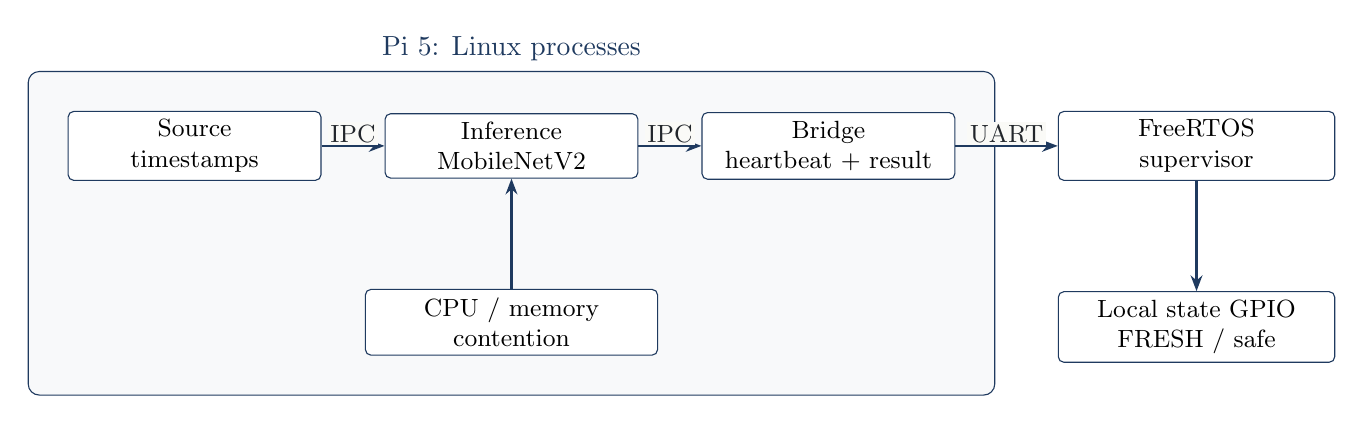
\begin{tikzpicture}[node distance=8mm]
\node[box,text width=30mm] (s) {Source\\timestamps};
\node[box,text width=30mm,right=of s] (i) {Inference\\MobileNetV2};
\node[box,text width=30mm,right=of i] (b) {Bridge\\heartbeat + result};
\node[box,text width=33mm,right=13mm of b] (m) {FreeRTOS\\supervisor};
\draw[flow] (s)--node[above,lbl]{IPC}(i);\draw[flow] (i)--node[above,lbl]{IPC}(b);
\draw[flow] (b)--node[above,lbl]{UART}(m);
\node[box,below=14mm of i,text width=35mm] (load) {CPU / memory\\contention};
\node[box,below=14mm of m,text width=33mm] (out) {Local state GPIO\\FRESH / safe};
\draw[flow] (load)--(i);\draw[flow] (m)--(out);
\begin{scope}[on background layer]\node[draw=navy,rounded corners,fill=navy!3,fit=(s)(i)(b)(load),inner sep=5mm,label={[navy]above:Pi 5: Linux processes}] {};\end{scope}
\end{tikzpicture}
\figcap{\label{fig:arch}A UART boundary separates Linux work from MCU judgment.}
\medskip\raggedright Figure~\ref{fig:arch} separates inter-process communication (IPC) from the UART serial link.
\takeaway{The STM32 supervises freshness independently of Linux scheduling.}
\end{frame}

\begin{frame}[t]{4. Scheduling and contention profiles}
\twocol{\textbf{Applied software-campaign profiles}\par\medskip
\begin{itemize}\item P0 source/bridge: OTHER, CPU 1, unlocked.\item P1 source/bridge: FIFO 60/70, CPU 1, memory locked.\item Both profiles: inference OTHER, CPU 0, unlocked.\end{itemize}
}{\textbf{Mechanisms and scope}\par\medskip
CPU (central processing unit) affinity controls placement.\par\medskip
\texttt{mlockall} locks resident memory.\par\medskip
Control groups (cgroups) can cap CPU service.\par\medskip
\textbf{PLANNED:} quota and packaged P3 kernel comparisons; no measured benefit.
}
\scope{[1] Linux scheduling. Applied E2 settings change priority and locking together. Cyclictest P1 is FIFO 50, a separate configuration. Loads and stressed cores: method, page 9.}
\takeaway{CPU priority and affinity do not isolate shared memory bandwidth.}
\end{frame}

\begin{frame}[t]{5. IPC and buffering policy}
Unix datagram sockets separate source, inference and bridge processes.
\par\bigskip\centering
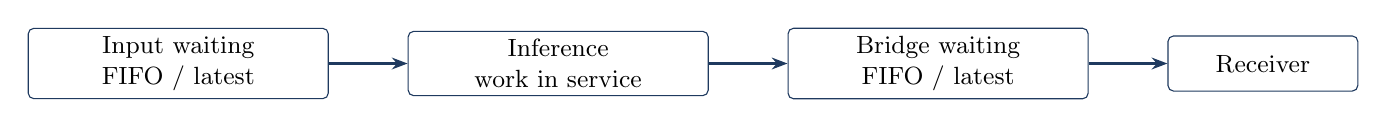
\begin{tikzpicture}[node distance=10mm]
\node[box,text width=36mm] (q) {Input waiting\\FIFO / latest};
\node[box,text width=36mm,right=of q] (i) {Inference\\work in service};
\node[box,text width=36mm,right=of i] (b) {Bridge waiting\\FIFO / latest};
\node[box,text width=22mm,right=of b] (rx) {Receiver};
\draw[flow](q)--(i);\draw[flow](i)--(b);\draw[flow](b)--(rx);
\end{tikzpicture}
\figcap{\label{fig:queues}Replacement acts only at its chosen waiting queue.}
\medskip\raggedright Figure~\ref{fig:queues}: bridge FIFO holds up to 256 results; latest keeps one unsent result.\par\medskip
Input latest drains waiting inputs before inference; it does not preempt current work.
\takeaway{Replacing after expensive work cannot remove a backlog before that work.}
\end{frame}

\begin{frame}[t]{6. Clocks and freshness}
\twocol{\textbf{One Pi clock per measurement}\par\medskip
\texttt{CLOCK\_MONOTONIC}: release deadlines.\par\medskip
\texttt{CLOCK\_MONOTONIC\_RAW}: recorded timestamps and age-at-send.\par\medskip
\textbf{Do not mix those timestamp domains.}\par\medskip
[2] Linux clock semantics.
}{\textbf{Independent MCU clock}\par\medskip
\(A_s=t_{send}-t_{input}\) on the Pi.\par\medskip
\(\widehat A=A_s+(t_{MCU}-t_{receipt})+B\).\par\medskip
\(B=5\) ms: configured transit allowance.\par\medskip
Echo exchange fits offset and drift [3].\par\medskip
Mapping uncertainty remains; no proven transit bound.
}
\takeaway{AoI is the age of the newest useful input at the consumer.}
\end{frame}

\begin{frame}[t]{7. Independent supervisor}
\centering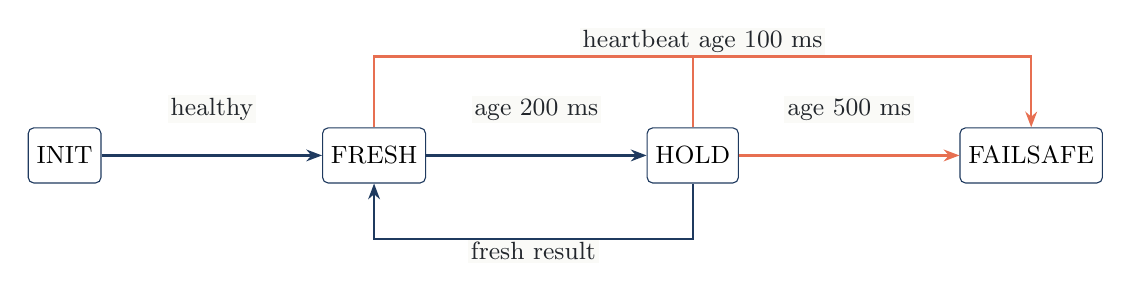
\begin{tikzpicture}[node distance=28mm]
\node[box] (init) {INIT};\node[box,right=of init] (fresh) {FRESH};\node[box,right=of fresh] (hold) {HOLD};\node[box,right=of hold] (fail) {FAILSAFE};
\draw[flow](init)--node[above=4mm,lbl]{healthy}(fresh);
\draw[flow](fresh)--node[above=4mm,lbl]{age 200 ms}(hold);
\draw[faultflow](hold)--node[above=4mm,lbl]{age 500 ms}(fail);
\draw[flow](hold.south) -- ++(0,-.7) -| node[pos=.25,below,lbl]{fresh result} (fresh.south);
\draw[faultflow](fresh.north) -- ++(0,.9) -| node[pos=.25,above,lbl]{heartbeat age 100 ms} (fail.north);
\coordinate (hbjoin) at ($(fresh.north)+(0,.9)$);
\draw[thick,color=fault](hold.north)--(hold.north |- hbjoin);
\end{tikzpicture}
\figcap{\label{fig:state}Separate timers test liveness and source freshness.}
\medskip\raggedright Figure~\ref{fig:state} uses configured, provisional thresholds.
\par\medskip FAILSAFE is latched. Portable core supports local healthy rearm (1 s); this port uses board reset.
\scope{FreeRTOS fixed-priority tasks [4]; single supervisor owner, static resources. No independent MCU hardware watchdog.}
\takeaway{A continuing heartbeat cannot make an old result fresh.}
\end{frame}

\begin{frame}[t]{8. Experimental method}
\twocol{\textbf{Retained rig}\par\medskip
Pi 5, 4 GB; Ubuntu 24.04.\par
Stock \texttt{6.8.0-1064-raspi} kernel.\par\smallskip
STM32F446RE; FreeRTOS.\par
USART1, 921600 baud; direct memory access (DMA) reception.\par\smallskip
3.3 V UART: Pi TX/RX \(\leftrightarrow\) PA10/PA9; shared ground.
}{\textbf{Load key (stress-ng on the Pi)}\par\medskip
CPU: compute workers, CPUs 2/3.\par
Stream: streaming arrays, CPU 2.\par
Cache: 2 MiB working set, CPU 2.\par
Memrate: read/write traffic, CPUs 2/3.\par\medskip
Timer: CPU 0; pipeline inference: CPU 0; source/bridge: CPU 1.
}
\medskip Cyclictest: 3\(\times\)120 s/cell; E1--E3: 3\(\times\)60 s/cell, pseudo-terminal (PTY).\par
Inference: 50 warm-ups + 1,000 calls/run; analyzer: 15 fault captures.
\scope{Performance governor: timer/pipeline; ondemand: model-only baseline (CPUs 0--3). PTY excludes physical UART/MCU. Exact load commands: CLAIMS.md.}
\takeaway{Keep timer, model, software pipeline and physical-fault scopes separate.}
\end{frame}

\begin{frame}[t]{9. Run validity and rule versions}
\begin{tabular}{@{}L{.32\linewidth}L{.28\linewidth}L{.32\linewidth}@{}}\toprule
Evidence & Stored v1 acceptance & Stricter v2 replay\\\midrule
Cyclictest & 30/30 & 6/30: idle only\\[5pt]
E1--E3, PTY & 45/45 & 0/45: RAW monitor times absent\\[5pt]
Original E4 entries & 17/25 & 17/25: unchanged\\\bottomrule
\end{tabular}\par
\bigskip
V2 requires whole-window RAW power timestamps, stressor liveness,\par
and clock fits no older than 5 s when mapping MCU time.
\scope{MEASURED v1 observations remain reported with their evidence limitation. Replay rejection is missing proof, not proof that every old run malfunctioned. [5] Results inventory.}
\takeaway{A measured number and a fully qualified comparison are different claims.}
\end{frame}

\begin{frame}[t]{10. Timer wake-up under contention}
\evidence{MEASURED -- v1; v2 accepts idle runs only}
\resultplot{cyclic}{Median run P99; 3 runs/cell, locked memory, CPU 0.}{Figure~\ref{fig:cyclic}: FIFO P99 rises from 9 to 239 \(\mu\)s under memrate.}
\scope{P0 OTHER / P1 FIFO 50. P50 gap includes timer slack; stressed v2 replay lacks recorded stressor liveness.}
\takeaway{Priority reduces CPU tails here; memory-contention tails remain.}
\end{frame}

\begin{frame}[t]{11. Inference baseline}
\evidence{MEASURED -- accepted subset of a mixed collection}
\resultplot{inference}{MobileNetV2 FP32, ONNX Runtime; inference only.}{Figure~\ref{fig:inference}: idle scaling does not predict loaded tails.}
\scope{21/24 accepted; idle reps 3/3/3/1, loaded 3/3/3/2. Three 4-thread runs excluded for live under-voltage. Ondemand; affinity CPUs 0--3.}
\takeaway{More model threads can compete with the stressed cores.}
\end{frame}

\begin{frame}[t]{12. E1: contention reaches the data path}
\evidence{MEASURED -- PTY, v1; 15/15 stored, 0/15 under v2 replay}
\resultplot{E1}{Input-to-Pi-reception P99; median across 3 runs.}{Figure~\ref{fig:E1}: memrate reaches 13,980 ms; idle is 48.47 ms.}
\scope{P0, performance governor. Service includes upstream waiting and pre/postprocessing; this is not model execution time. Logarithmic axis.}
\takeaway{The memory-loaded pipeline accumulates seconds of waiting.}
\end{frame}

\begin{frame}[t]{13. E2: runtime tuning has limits}
\evidence{MEASURED -- PTY, v1; 18/18 stored, 0/18 under v2 replay}
\resultplot{E2}{Matched loads; P99 of delivery, median across 3 runs.}{Figure~\ref{fig:E2}: memrate P99 stays 13,260 / 12,890 ms for P0 / P1.}
\scope{P0 source/bridge: CPU 1, unlocked. P1: FIFO 60/70, CPU 1, locked. Both: inference OTHER, CPU 0, unlocked. This compares profiles, not scheduling class alone.}
\takeaway{P1 does not remove memory-loaded backlog or improve every cache result.}
\end{frame}

\begin{frame}[t]{14. E3: queue observations and interpretation}
\evidence{MEASURED -- PTY, v1; 12/12 stored, 0/12 under v2 replay}
\resultplot{E3}{Initialized time-average AoI; stalls and final tail included.}{Figure~\ref{fig:E3}: loaded bridge FIFO/latest average ages are 6,660 / 6,958 ms.}
\scope{MEASURED v1: zero bridge replacements; 100 ms inputs; 122--130 ms completion intervals. FLAGGED E3b: input-latest P99 254--268 ms vs FIFO 13.8--15.9 s; all loaded runs power-invalid.}
\takeaway{INFERRED: backlog before inference. Clean input-policy benefit: UNKNOWN.}
\end{frame}

\begin{frame}[t]{15. E4: interpret the transition reason}
\evidence{MEASURED -- accepted MCU transitions; short-window scopes differ}
\resultplot[48mm]{E4}{One point per accepted run; horizontal offsets separate close samples.}{Figure~\ref{fig:E4}: reason 3 uses heartbeat; reasons 9/10 use inference.}
\scope{F1 kill, F2 bridge stop, F3 inference stop, F4 FIFO-99 hog, F5 inference suppression. Accepted F1/F2/F3/F5: 5 each; F4: 7/14. F4 first events mix reasons 9 and 3.}
\takeaway{About 175/475 ms after receipt matches 200/500 ms source-age thresholds.}
\end{frame}

\begin{frame}[t]{16. Independent analyzer cross-check}
\evidence{MEASURED -- retained physical captures; collection remains FLAGGED}
\(\Delta=L-M\); positive means the analyzer interval is longer.\par
\(L\): last physical UART byte end \(\to\) both PA5/PB5 low.\par
\(M\): last accepted heartbeat receipt \(\to\) FAILSAFE STATE\_EVENT time.
\par\smallskip
\resultplot[36mm]{LA}{Residuals by capture index; full IDs in qa/LA\_capture\_key.md.}{Figure~\ref{fig:LA}: 10/15 final HEARTBEAT references give +47.5--67.6 \(\mu\)s.}
\scope{Residual includes timestamp placement, reception/output delay and clock effects. Other 5 end with INFERENCE/ECHO. 8 MHz sampling; absolute calibration UNKNOWN.}
\takeaway{Matching frame types aid comparison; they do not qualify the FLAGGED collection.}
\end{frame}

\begin{frame}[t]{17. Limitations}
\begin{itemize}
\item 5 V / 3 A supply; live under-voltage excludes loaded runs.
\item Original real-UART E3: 18/18 FLAGGED; no clean physical AoI.
\item V2 replay exposes missing monitor timestamps and stressor proof.
\item Small samples and observed maxima are not worst-case bounds.
\item Firmware review fixes compile; they are \textbf{not re-flashed or rig-verified}.
\end{itemize}
\scope{Analyzer captures add a GPIO observation to the older stage report; they do not close transit, oscillator, rearm or watchdog qualification.}
\takeaway{The evidence supports this experimental envelope, with explicit exclusions.}
\end{frame}

\begin{frame}[t]{18. Conclusion and contributions}
\begin{itemize}
\item \textbf{Timing:} priority improves observed timer tails; shared contention persists.
\item \textbf{Freshness:} upstream backlog is INFERRED from measured queue behavior.
\item \textbf{Supervision:} independent MCU timers separate stale work from silence.
\item \textbf{Artifact:} shared protocol, instrumented pipeline, raw data and exclusions.
\end{itemize}
\bigskip
Clean input-policy benefit remains \textbf{UNKNOWN}; loaded E3b is \textbf{FLAGGED}.\par\medskip
The teaching result connects scheduling, IPC, clocks and real-time state decisions.
\takeaway{Defensible measurements include the failures and the limits of each claim.}
\end{frame}

\begin{frame}[t]{19. Future work}
\evidence{PLANNED}
\begin{itemize}
\item Restore clean power; rerun input-policy and physical E3 under v2.
\item Flash reviewed firmware; verify DMA, stack margins and event logging.
\item Match analyzer references; calibrate clocks, transit and rearm margins.
\item Extend fault exposure and recovery; reach five valid repeats per cell.
\end{itemize}
\bigskip
Quota and packaged P3 kernel comparisons remain optional matched experiments.
\takeaway{The next deliverable is qualified physical freshness evidence.}
\end{frame}

\begin{frame}[t]{20. References}
\begin{enumerate}
\item Linux man-pages. \href{https://man7.org/linux/man-pages/man7/sched.7.html}{\textit{sched(7)}}: scheduling policies and affinity.
\item Linux man-pages. \href{https://man7.org/linux/man-pages/man2/clock_gettime.2.html}{\textit{clock\_gettime(2)}}: monotonic and raw clocks.
\item D. Mills. \href{https://www.rfc-editor.org/rfc/rfc4330}{\textit{RFC 4330}}, January 2006, section 5: four-timestamp math.
\item FreeRTOS. \href{https://www.freertos.org/Documentation/02-Kernel/02-Kernel-features/01-Tasks-and-co-routines/00-Tasks-and-co-routines}{\textit{Tasks and Co-routines}}: kernel task model.
\item Project artifact. \textit{STAGE\_REPORT.md}, \textit{results/README.md},\par
retained data (11--12 October 2026); source snapshot \texttt{5e3f461}.
\end{enumerate}
\scope{Primary documentation checked 13 October 2026. Exact figure inputs and hashes: qa/source\_hashes.json. Slide-to-evidence mapping: CLAIMS.md.}
\end{frame}

\appendix
\begin{frame}[c]\centering{\Huge\bfseries\color{navy}Backup\par}\medskip Questions, evidence and configuration detail\end{frame}

\begin{frame}[t]{B1. UART protocol frame}
\centering\begin{tabular}{@{}lrrrrrr@{}}\toprule
Field & SOF & Version & Type & Seq & Length & Payload + CRC\\\midrule
Bytes & 2 & 1 & 1 & 2 & 1 & 0--64 + 2\\\bottomrule
\end{tabular}\par\par\bigskip\raggedright
\begin{itemize}\item SOF: A5 5A; little-endian fields; version 3 encoder.\item CRC-16/CCITT-FALSE checks version through payload.\item INFERENCE: 35 bytes, including age-at-send.\item HEARTBEAT carries session identity; STATE\_EVENT carries reason.\end{itemize}
\scope{CALCULATED: 35 bytes \(\times\) 10 bits / 921600 baud = 0.380 ms nominal line time. This excludes all software delay. Source: protocol/PROTOCOL.md.}
\takeaway{Integrity, sequence and freshness checks serve different purposes.}
\end{frame}

\begin{frame}[t]{B2. Clock math and measurement boundaries}
\(T_1,T_4\): Pi; \(T_2,T_3\): MCU, in microseconds.\par\medskip
\[O=\frac{(T_2-T_1)+(T_3-T_4)}{2},\qquad d=(T_4-T_1)-(T_3-T_2)\]
\[O(t)=O_R+D(t-R),\qquad t_{Pi}=R+\frac{t_{MCU}-R-O_R}{1+D}\]
\begin{itemize}\item Asymmetric delays bias offset; fit residual is not absolute accuracy.\item V2 rejects fits older than 5 s; accepted RMS ceiling is 200 \(\mu\)s.\item Held-value AoI integrates age over initialized time, including final tail.\end{itemize}
\scope{[3] RFC 4330, section 5; protocol/CLOCK\_SYNC.md. RMS ceiling is a configured acceptance choice.}
\end{frame}

\begin{frame}[t]{B3. Threshold rationale and rearm}
\begin{tabular}{@{}L{.24\linewidth}L{.17\linewidth}L{.51\linewidth}@{}}\toprule
Timer & Configured & Retained observation\\\midrule
Heartbeat & 100 ms & F1/F2 reason 3: 100.128--100.641 ms\\[5pt]
Source HOLD & 200 ms & F5 reason 9: 174.950--175.917 ms after receipt\\[5pt]
Source FAILSAFE & 500 ms & F5 reason 10: 474.950--475.917 ms after receipt\\[5pt]
Healthy rearm & 1,000 ms & Core supports it; board port requires reset\\[5pt]
Transit allowance & 5 ms & Provisional; no validated upper bound\\\bottomrule
\end{tabular}\par
\bigskip Result age also includes age-at-send: receipt elapsed is not source age.
\scope{Configured values are ASSUMED choices, not calibrated safety budgets. main.c; supervisor.c; raw F5 events. E4 threshold snapshots are empty/null.}
\takeaway{Healthy heartbeat alone cannot clear latched FAILSAFE.}
\end{frame}

\begin{frame}[t]{B4. Full run-validity inventory}
\begin{tabular}{@{}L{.40\linewidth}L{.15\linewidth}L{.36\linewidth}@{}}\toprule
Collection & Accepted & Scope / qualification\\\midrule
Cyclictest & 30/30 v1 & v2: 6/30, idle only\\[3pt]
Inference baseline & 21/24 & Mixed; three live under-voltage exclusions\\[3pt]
E1 / E2 / E3 & 15 / 18 / 12 & v1 PTY; v2: 0/45\\[3pt]
E3b input policy & 3/12 & All six loaded runs FLAGGED\\[3pt]
Real-UART E3 (original / rerun) & 0/18 each & All FLAGGED; distinct validity rules\\[3pt]
Original E4 & 17/25 entries & 20 performed; 5 F5 unperformed\\[3pt]
Extra F4 / later F5 & 5/9 / 5/5 & Short-window transition checks\\[3pt]
Logic analyzer & 15 captures & FLAGGED collection; 1 incomplete attempt\\\bottomrule
\end{tabular}\par
\scope{Source: results/README.md. Missing STATE\_EVENT alone cannot prove unhealthy steady state. No excluded observation is promoted into a clean comparison.}
\end{frame}

\begin{frame}[t]{B5. Full E4 table: MCU-local timing}
\evidence{MEASURED -- milliseconds; nearest-rank P50 / P95 / max}
\centering\begin{tabular}{@{}lrrr@{}}\toprule Fault & Valid & First P50 / P95 / max & FAILSAFE P50 / P95 / max\\\midrule
F1 & 5/5 & 175.317 / 175.535 / 175.535 & 100.456 / 100.641 / 100.641\\[5pt]
F2 & 5/5 & 175.206 / 175.709 / 175.709 & 100.577 / 100.596 / 100.596\\[5pt]
F3 & 5/5 & 175.754 / 175.815 / 175.815 & 475.754 / 475.815 / 475.815\\[5pt]
F4 & 7/14 & 100.639 / 175.229 / 175.229 & 100.556 / 100.931 / 100.931\\[5pt]
F5 & 5/5 & 175.596 / 175.917 / 175.917 & 475.596 / 475.917 / 475.917\\[5pt]
\bottomrule\end{tabular}
\par\bigskip\raggedright
F1/F2: first 9, FAILSAFE 3.\par\medskip F3/F5: first 9, FAILSAFE 10. F4: six direct 3; one first 9.
\scope{F4 combines original 2/5 with extra 5/9; short windows differ. Reasons 9/10 reference INFERENCE; reason 3 references HEARTBEAT. P95 = maximum at these sample sizes.}
\takeaway{A mixed-reference first-transition summary is not heartbeat latency.}
\end{frame}

\begin{frame}[t]{B6. Full E4 table: mapped fault-onset timing}
\evidence{MEASURED -- milliseconds; nearest-rank P50 / P95 / max}
\centering\begin{tabular}{@{}lrrr@{}}\toprule Fault & Valid & First P50 / P95 / max & FAILSAFE P50 / P95 / max\\\midrule
F1 & 5/5 & 83.342 / 83.561 / 83.561 & 85.357 / 86.209 / 86.209\\[5pt]
F2 & 5/5 & 83.151 / 83.715 / 83.715 & 85.715 / 86.113 / 86.113\\[5pt]
F3 & 5/5 & 83.646 / 85.914 / 85.914 & 383.620 / 385.888 / 385.888\\[5pt]
F4 & 7/14 & 85.625 / 87.871 / 87.871 & 87.277 / 97.344 / 97.344\\[5pt]
F5 & 5/5 & 83.608 / 85.563 / 85.563 & 383.603 / 385.558 / 385.558\\[5pt]
\bottomrule\end{tabular}
\par\bigskip\raggedright
Mapped intervals begin at Pi software fault onset, through the echo estimator.\par\medskip
MCU-local intervals begin at the last accepted message selected by reason.\par\medskip
Accepted runs record zero false transitions in their checked pre-fault windows.
\scope{Clock residual and timestamp placement limit mapping accuracy. Extra F4 and F5 do not qualify original recovery/long-exposure gates. No false-trip rate or worst-case bound follows.}
\end{frame}

\begin{frame}[t]{B7. Claim-to-evidence map}
\begin{tabular}{@{}L{.35\linewidth}L{.26\linewidth}L{.31\linewidth}@{}}\toprule
Claim & Evidence label & Retained source\\\midrule
FIFO timer tails differ & MEASURED v1 & cyclictest summaries\\[5pt]
Memory-loaded backlog & MEASURED v1, PTY & E1/E2 tables, infer.csv\\[5pt]
Zero replacements; slow completions & MEASURED v1, PTY & E3 table; infer.csv\\[5pt]
Backlog before inference & INFERRED & E3 queue observations\\[5pt]
Clean input-latest benefit & UNKNOWN; E3b FLAGGED & Power-invalid E3b logs\\[5pt]
Heartbeat / source-age decisions & MEASURED, scoped & E4/F5 STATE\_EVENT\\[5pt]
10/15 matching analyzer references & CALCULATED; collection FLAGGED & VCD + CRC decode + events\\[5pt]
Clean physical AoI / safety bound & UNKNOWN & Not established\\\bottomrule
\end{tabular}\par
\scope{Analyzer: calculated comparison of retained MEASURED captures; matching frame types do not establish run validity. Full qualifications: CLAIMS.md; hashes: qa/source\_hashes.json.}
\end{frame}

\begin{frame}[t]{B8. Tools and branch map}
\twocol{\textbf{Execution environment}\par\medskip
Mac: XeLaTeX, plots, cross-compile, flash.\par\medskip
Pi: Linux pipeline, stress-ng, cyclictest, metadata.\par\medskip
STM32: FreeRTOS tasks, TIM2, DMA UART, state GPIO.\par\medskip
Analysis: e\_summary, e4\_summary, la\_analyze.
}{\textbf{Artifact provenance}\par\medskip
\texttt{feat/pi-timing-tools}\par
\texttt{feat/inference-baseline}\par
\texttt{feat/fw-rx-fix}\par
\(\downarrow\) merged release evidence\par
\texttt{release/os-final}\par
\(\downarrow\) submission worktree\par
\texttt{feat/os-submission} / \texttt{5e3f461}
}
\scope{Branch history is provenance, not a completion claim. This deck build changes only submission/defense; it runs no hardware experiments.}
\takeaway{Regenerate this deck with its retained script and source manifest.}
\end{frame}
\end{document}
